\documentclass[a4paper, 12pt]{article}

\usepackage[utf8]{inputenc}
\usepackage[T1]{fontenc}
\usepackage[french]{babel}
\usepackage[top=2cm, bottom=2cm, left=1.5cm, right=1.5cm,headheight=16pt]{geometry}
\usepackage{lmodern}

\addto\captionsfrench{%
    \renewcommand{\tablename}{\textsc{Tableau}}%
}

\usepackage{cover-page}
\title{Finite State Transducers Just-In-Time Compiling}
\subtitle{Do you hear the bytecode ?}
\author{Émilien Boulben\\Victor Delepine\\Corentin Peuvrel}
\location{Paris}
\date{\today}
\blurb
{
    Institut Supérieur d'Électronique de Paris\\
    \textbf{Projet de Fin d'Études}\\
    ~\\
    Reponsable: M. Hugueney
}

\usepackage{fancy-perso}
\usepackage{lastpage}
\headerleft{Finite State Transducer Just-In-Time Compiling}
\headerright{Institut Superieur d'Électronique de Paris}
\footerleft{É.Boulben, V.Delepine, C.Peuvrel}
\footerright{\hyperlink{Contents}{Table des matières}}

\usepackage{parskip}
\setlength{\parindent}{18pt}

\usepackage{listings}
\usepackage{upquote}
\usepackage{graphicx}
\usepackage{listings}
\usepackage{xcolor}

\makeatletter
\newcommand{\lstdefinestylecustom}[3] {%
    \ifnum\pdfstrcmp{#3}{x86masm}=0
    \lstdefinestyle{#1}{
        numbers=left,
        stepnumber=1,
        numberstyle=\scriptsize,
        belowcaptionskip=1\baselineskip,
        captionpos=b,
        breaklines=true,
        frame=L,
        xleftmargin=\parindent,
        language=[#3]#2,
        showstringspaces=false,
        basicstyle=\footnotesize\ttfamily,
        keywordstyle=\bfseries\color{green!40!black},
        commentstyle=\itshape\color{purple!40!black},
        identifierstyle=\color{blue},
        stringstyle=\color{orange},
        comment=[l]\#,
    }
    \else
    \lstdefinestyle{#1}{
        numbers=left,
        stepnumber=1,
        numberstyle=\scriptsize,
        belowcaptionskip=1\baselineskip,
        captionpos=b,
        breaklines=true,
        frame=L,
        xleftmargin=\parindent,
        language=#2,
        showstringspaces=false,
        basicstyle=\footnotesize\ttfamily,
        keywordstyle=\bfseries\color{green!40!black},
        commentstyle=\itshape\color{purple!40!black},
        identifierstyle=\color{blue},
        stringstyle=\color{orange},
    }
    \fi
}
\makeatother

\lstdefinestylecustom{custombash}{bash}{}
\lstdefinestylecustom{customc}{C}{}
\lstdefinestylecustom{customasm}{Assembler}{x86masm}

\usepackage[pdftex,breaklinks,linktocpage,unicode]{hyperref}
\hypersetup{
    unicode=false,          % non-Latin characters in Acrobat’s bookmarks
    pdftoolbar=true,        % show Acrobat’s toolbar?
    pdfmenubar=true,        % show Acrobat’s menu?
    pdffitwindow=false,     % window fit to page when opened
    pdfstartview={FitH},    % fits the width of the page to the window
    pdftitle={Finite State Transducer Just-In-Time Compiling},    % title
    pdfauthor={Émilien Boulben, Victor Delépine, Corentin Peuvrel},     % author
    pdfsubject={FST, bytecode, optimisation},   % subject of the document
    pdfcreator={Émilien Boulben},   % creator of the document
    pdfproducer={Émilien Boulben}, % producer of the document
    pdfkeywords={FST, assembler, bytecode, just, time, java}, % list of keywords
    pdfnewwindow=true,      % links in new window
    colorlinks=true,       % false: boxed links; true: colored links
    linkcolor=black,          % color of internal links (change box
    % color with linkbordercolor)
    linktoc=all,
    citecolor=green,        % color of links to bibliography
    filecolor=magenta,      % color of file links
    urlcolor=cyan           % color of external links
}


\begin{document}

\maketitle

\newpage
\clearpage
\pagenumbering{Roman}
\setcounter{page}{1}
\footercenter{\textbf{\thepage}}
\fancyperso{HL}{HR}{FL}{FC}{}

\hypertarget{Contents}{}
\tableofcontents
\newpage
\lstlistoflistings
\newpage
\listoftables
\newpage
\listoffigures

\newpage
\clearpage
\pagenumbering{arabic}
\setcounter{page}{1}
\footercenter{\textbf{Page \thepage/\pageref{LastPage}}}
\fancyperso{HL}{HR}{FL}{FC}{FR}

\section*{Introduction}
\addcontentsline{toc}{section}{\protect\numberline{}Introduction}

\newpage
\section{Analyse préalable}

\newpage
\section{Des FST en JIT}

\newpage
\section{Optimiser : comment ?}

\newpage
\section*{Conclusion}
\addcontentsline{toc}{section}{\protect\numberline{}Conclusion}

\newpage
\appendix
\section{Annexe : tests avec un script shell}

\subsection{Dictionnaires}

\begin{table}[h]
    \centering
    \begin{tabular}{|l|l|}
        \hline
        Value & Word \\
        \hline
        0 & mop \\
        1 & moth \\
        2 & pop \\
        3 & star \\
        4 & stop \\
        5 & top \\
        \hline
    \end{tabular}
    \caption{Dictionnaire à utiliser avec la FST dans le \autoref{tab:fst1}}
    \label{tab:dico1}
\end{table}

\begin{table}[h]
    \centering
    \begin{tabular}{|l|l|}
        \hline
        Value & Word \\
        \hline
        0 & mop \\
        1 & moth \\
        2 & pop \\
        3 & slop \\
        4 & sloth \\
        5 & stop \\
        6 & top \\
        \hline
    \end{tabular}
    \caption{Dictionnaire à utiliser avec la FST dans le \autoref{tab:fst2}}
    \label{tab:dico2}
\end{table}

\clearpage
\subsection{FST}

\begin{table}[ht]
    \centering
    \begin{tabular}{|l||c|c|c|c|c|c|c|c|c|c|c|c|c|c|c|}
        \hline
        N\oe u & 0 & 0 & 0 & 0 & 1 & 2 & 3 & 2 & 4 & 6 & 7 & 5 & 7 & 8 & \\ \hline
        N\oe u suivant & 1 & 4 & 4 & 6 & 2 & 3 & 9 & 9 & 5 & 7 & 5 & 9 & 8 & 9 & \\ \hline
        N\oe u final &&&&&&&&&&&&&&& 9 \\ \hline
        Caractère & M & P & T & S& O & T & H & P & O & T & O & P & A & R & \\ \hline
        Poids & & 2 & 5 & 3 &&& 1 &&&&1&&&& \\ \hline
    \end{tabular}
    \caption{FST utilisée avec le dictionnaire \autoref{tab:dico1}, voir \autoref{fig:fst-dico1} page \pageref{fig:fst-dico1}}
    \label{tab:fst1}
\end{table}

\begin{figure}[ht]
    \centering
    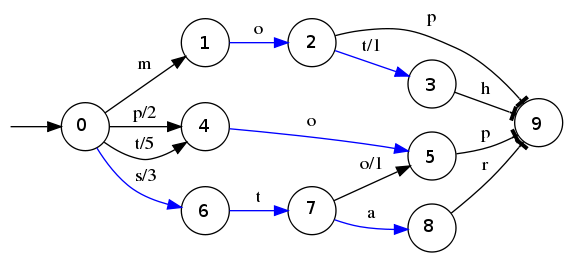
\includegraphics[scale=0.5]{../c_asm/1.png}
    \caption{La FST associée avec le \autoref{tab:fst1} page \pageref{tab:fst1}}
    \label{fig:fst-dico1}
\end{figure}

\begin{table}[ht]
    \centering
    \begin{tabular}{|l||c|c|c|c|c|c|c|c|c|c|c|c|c|c|c|}
        \hline
        N\oe u & 0 & 0 & 0 & 0 & 3 & 3 & 1 & 2 & 4 & 5 & 6 & 5 &\\ \hline
        N\oe u suivant & 1 & 1 & 3 & 4 & 1 & 4 & 2 & 7 & 5 & 6 & 7 & 7 &\\ \hline
        N\oe u final &&&&&&&&&&&&& 7 \\ \hline
        Caractère & P & T & S & M& T & L & O & P & O & T & H & P & \\ \hline
        Poids & 2 & 6 & 3 &  & 2 & & & & & 1 &&& \\ \hline
    \end{tabular}
    \caption{FST utilisée avec le dictionnaire \autoref{tab:dico2}, voir \autoref{fig:fst-dico2} page \pageref{fig:fst-dico2}}
    \label{tab:fst2}
\end{table}

\begin{figure}[!htb]
    \centering
    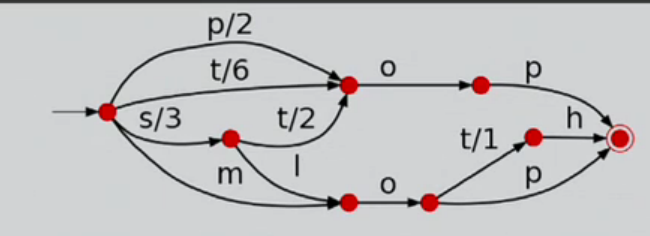
\includegraphics[scale=0.5]{../c_asm/2.png}
    \caption{La FST associée avec le \autoref{tab:fst2} page \pageref{tab:fst2}}
    \label{fig:fst-dico2}
\end{figure}

\clearpage
\subsection{Générer à la volée du code C}
\subsubsection{Script shell}

\lstinputlisting[style=custombash, caption=Script pour générer un code C à la volée d'une FST,label=lst:bashgen]{../c_asm/gen.sh}

\clearpage
\subsubsection{Code C généré pour la FST définie dans le \autoref{tab:fst1}}

\lstinputlisting[style=customc, caption=Code C généré pour la FST définie dans \autoref{tab:fst1},label=lst:cfst1]{../c_asm/gen_c_fst1.c}

\clearpage
\subsubsection{Code C généré pour la FST définie dans le \autoref{tab:fst2}}

\lstinputlisting[style=customc, caption=Code C généré pour la FST définie dans \autoref{tab:fst2},label=lst:cfst2]{../c_asm/gen_c_fst2.c}


\clearpage
\subsection{Générer à la volée du code assembleur x86}
\subsubsection{Script shell}

\lstinputlisting[style=custombash, caption=Script pour générer un code assembleur x86 à la colée d'une FST, label=lst:bashgenasm]{../c_asm/gen_asm.sh}

\clearpage
\subsubsection{Code assembleur x86 généré pour la FST définié dans le \autoref{tab:fst1}}

\lstinputlisting[style=customasm, caption=Code assembleur x86 généré pour la FST définie dans \autoref{tab:fst1}, label=lst:asmfst1]{../c_asm/gen_asm_fst1.asm}

\clearpage
\subsubsection{Code assembleur x86 généré pour la FST définié dans le \autoref{tab:fst2}}

\lstinputlisting[style=customasm, caption=Code assembleur x86 généré pour la FST définie dans \autoref{tab:fst2}, label=lst:asmfst2]{../c_asm/gen_asm_fst2.asm}

\end{document}
